\documentclass[sigplan, anonymous, review]{acmart}

\usepackage{booktabs} % For formal tables
\usepackage{listings}


% Copyright
%\setcopyright{none}
%\setcopyright{acmcopyright}
%\setcopyright{acmlicensed}
\setcopyright{rightsretained}
%\setcopyright{usgov}
%\setcopyright{usgovmixed}
%\setcopyright{cagov}
%\setcopyright{cagovmixed}


% DOI
\acmDOI{10.475/123_4}

% ISBN
\acmISBN{123-4567-24-567/08/06}

%Conference
\acmConference[WOODSTOCK'97]{ACM Woodstock conference}{July 1997}{El
  Paso, Texas USA}
\acmYear{1997}
\copyrightyear{2016}

\acmPrice{15.00}

%\acmBadgeL[http://ctuning.org/ae/ppopp2016.html]{ae-logo}
%\acmBadgeR[http://ctuning.org/ae/ppopp2016.html]{ae-logo}

% Submission ID
\acmSubmissionID{123-A56-BU3}


\begin{document}
\title{Software Restoration of Legacy-Parallel Pthreads Parallel Applications}
\titlenote{Produces the permission block, and
  copyright information}
\subtitle{Extended Abstract}
%\subtitlenote{The full version of the author's guide is available as
  %\texttt{acmart.pdf} document}

\author{Discovery St Andrews People}
\authornote{Some note about Discovery People}
\orcid{1234-5678-9012}
\affiliation{%
  \institution{Institute for Clarity in Documentation}
  \streetaddress{P.O. Box 1212}
  \city{Dublin}
  \state{Ohio}
  \postcode{43017-6221}
}
\email{trovato@corporation.com}

%\author{G.K.M. Tobin}
%\authornote{The secretary disavows any knowledge of this author's actions.}
%\affiliation{%
%  \institution{Institute for Clarity in Documentation}
%  \streetaddress{P.O. Box 1212}
%  \city{Dublin}
%  \state{Ohio}
%  \postcode{43017-6221}
%}
%\email{webmaster@marysville-ohio.com}

%% \author{Aparna Patel}
%% \affiliation{%
%%  \institution{Rajiv Gandhi University}
%%  \streetaddress{Rono-Hills}
%%  \city{Doimukh}
%%  \state{Arunachal Pradesh}
%%  \country{India}}
%% \author{Huifen Chan}
%% \affiliation{%
%%   \institution{Tsinghua University}
%%   \streetaddress{30 Shuangqing Rd}
%%   \city{Haidian Qu}
%%   \state{Beijing Shi}
%%   \country{China}}

%% \author{Charles Palmer}
%% \affiliation{%
%%   \institution{Palmer Research Laboratories}
%%   \streetaddress{8600 Datapoint Drive}
%%   \city{San Antonio}
%%   \state{Texas}
%%   \postcode{78229}}
%% \email{cpalmer@prl.com}

%% \author{John Smith}
%% \affiliation{\institution{The Th{\o}rv{\"a}ld Group}}
%% \email{jsmith@affiliation.org}

%% \author{Julius P.~Kumquat}
%% \affiliation{\institution{The Kumquat Consortium}}
%% \email{jpkumquat@consortium.net}


% The default list of authors is too long for headers.
\renewcommand{\shortauthors}{Discovery et al.}



\begin{abstract}
  This paper describes pattern discovery mechanisms developed in the Discovery project. 
\end{abstract}

%
% The code below should be generated by the tool at
% http://dl.acm.org/ccs.cfm
% Please copy and paste the code instead of the example below.
%
%\begin{CCSXML}
%<ccs2012>
% <concept>
%  <concept_id>10010520.10010553.10010562</concept_id>
%  <concept_desc>Computer systems organization~Embedded systems</concept_desc>
%  <concept_significance>500</concept_significance>
% </concept>
% <concept>
%  <concept_id>10010520.10010575.10010755</concept_id>
%  <concept_desc>Computer systems organization~Redundancy</concept_desc>
%  <concept_significance>300</concept_significance>
% </concept>
% <concept>
%  <concept_id>10010520.10010553.10010554</concept_id>
%  <concept_desc>Computer systems organization~Robotics</concept_desc>
%  <concept_significance>100</concept_significance>
% </concept>
% <concept>
%  <concept_id>10003033.10003083.10003095</concept_id>
%  <concept_desc>Networks~Network reliability</concept_desc>
%  <concept_significance>100</concept_significance>
% </concept>
%</ccs2012>
%\end{CCSXML}

%\ccsdesc[500]{Computer systems organization~Embedded systems}
%\ccsdesc[300]{Computer systems organization~Redundancy}
%\ccsdesc{Computer systems organization~Robotics}
%\ccsdesc[100]{Networks~Network reliability}


\keywords{ACM proceedings, \LaTeX, text tagging}

%\begin{teaserfigure}
%  \includegraphics[width=\textwidth]{sampleteaser}
%  \caption{This is a teaser}
%  \label{fig:teaser}
%\end{teaserfigure}


\maketitle

\section{Introduction}

\noindent
Parallel patterns are well established high-level parallel programming model for producing portable, maintainable, adaptive and efficient parallel code. They have been endorsed by some of the biggest IT companies, such as Intel and Microsoft, who have developed their own parallel pattern libraries (Intel TBB, Microsoft PPL etc.) A standard way of using these libraries is to start with the sequential code, identify in it the portions of the code that are amenable to parallelisation together with the exact parallel pattern to be applied, and then instantiating the identified pattern at the identified location in the code, after possibly restructuring the code to accommodate for parallelism. Sequential code gives the cleanest starting point for introduction of parallel patterns. There exists, however, a large base of \emph{legacy} code that was parallelised using lower-level, mostly ad-hoc parallelisation methods and libraries, such as \lstinline{pThreads}. This code is usually tailored to a specific parallelisation, all but preventing exploration of alternative parallelisation methods, and optimised for a specific system architecture. All this significantly reduces maintainability and portability of the code. %with highly-specific and tuned data structures which prevent alternative (possibly more efficient parallelisations) or portability to different platforms. Also, code maintainance requires intricate knowledge about the system architecture and various low-level underlying mechanisms such as thread creation, synchronisation and scheduling. 
Introducing structured parallelism in form of instances of parallel patterns into legacy-parallel code would significantly improve the code with respect to maintainability and portability. This is, however, usually a daunting task due to various factors, such as high degree of specialisation and custom tuning of the legacy code, incompability between lstinline{pThreads} and parallel pattern libraries, usage of very specific, custom-built data structures tailored to a specific parallelism model etc.
  
This paper presents a first step towards a semi-automated \emph{software restoration} methodology of restructuring and refactoring legacy-parallel code into structured, pattern-based parallel programs. The focus of the paper is on software refactorings to semi-automatically \emph{eliminate} parallelism from a parallel application written using the \lstinline{pthreads} library. This turns the legacy-parallel code into "unclean" sequential (or possibly concurrent) code, which does not contain parallelism, but which might still have some parallelism-specific variables and/or data structures. We demonstrate, on a number of legacy-parallel applications, that after applying parallelism removal refactorings, it is possible to obtain structured parallel code that behaves better than the original legacy-parallel version (in terms of e.g.~performance, portability or maintainability).

This paper makes the following specific research contributions:
\begin{itemize}
    \item XX
    \item XX
\end{itemize}

\section{Background}
\subsection{Parallel Patterns and Libraries}
\subsection{Pattern Discovery}
\subsection{Refactoring for Parallelism}

\section{Software Restoration}

\begin{figure}
  \begin{center}
    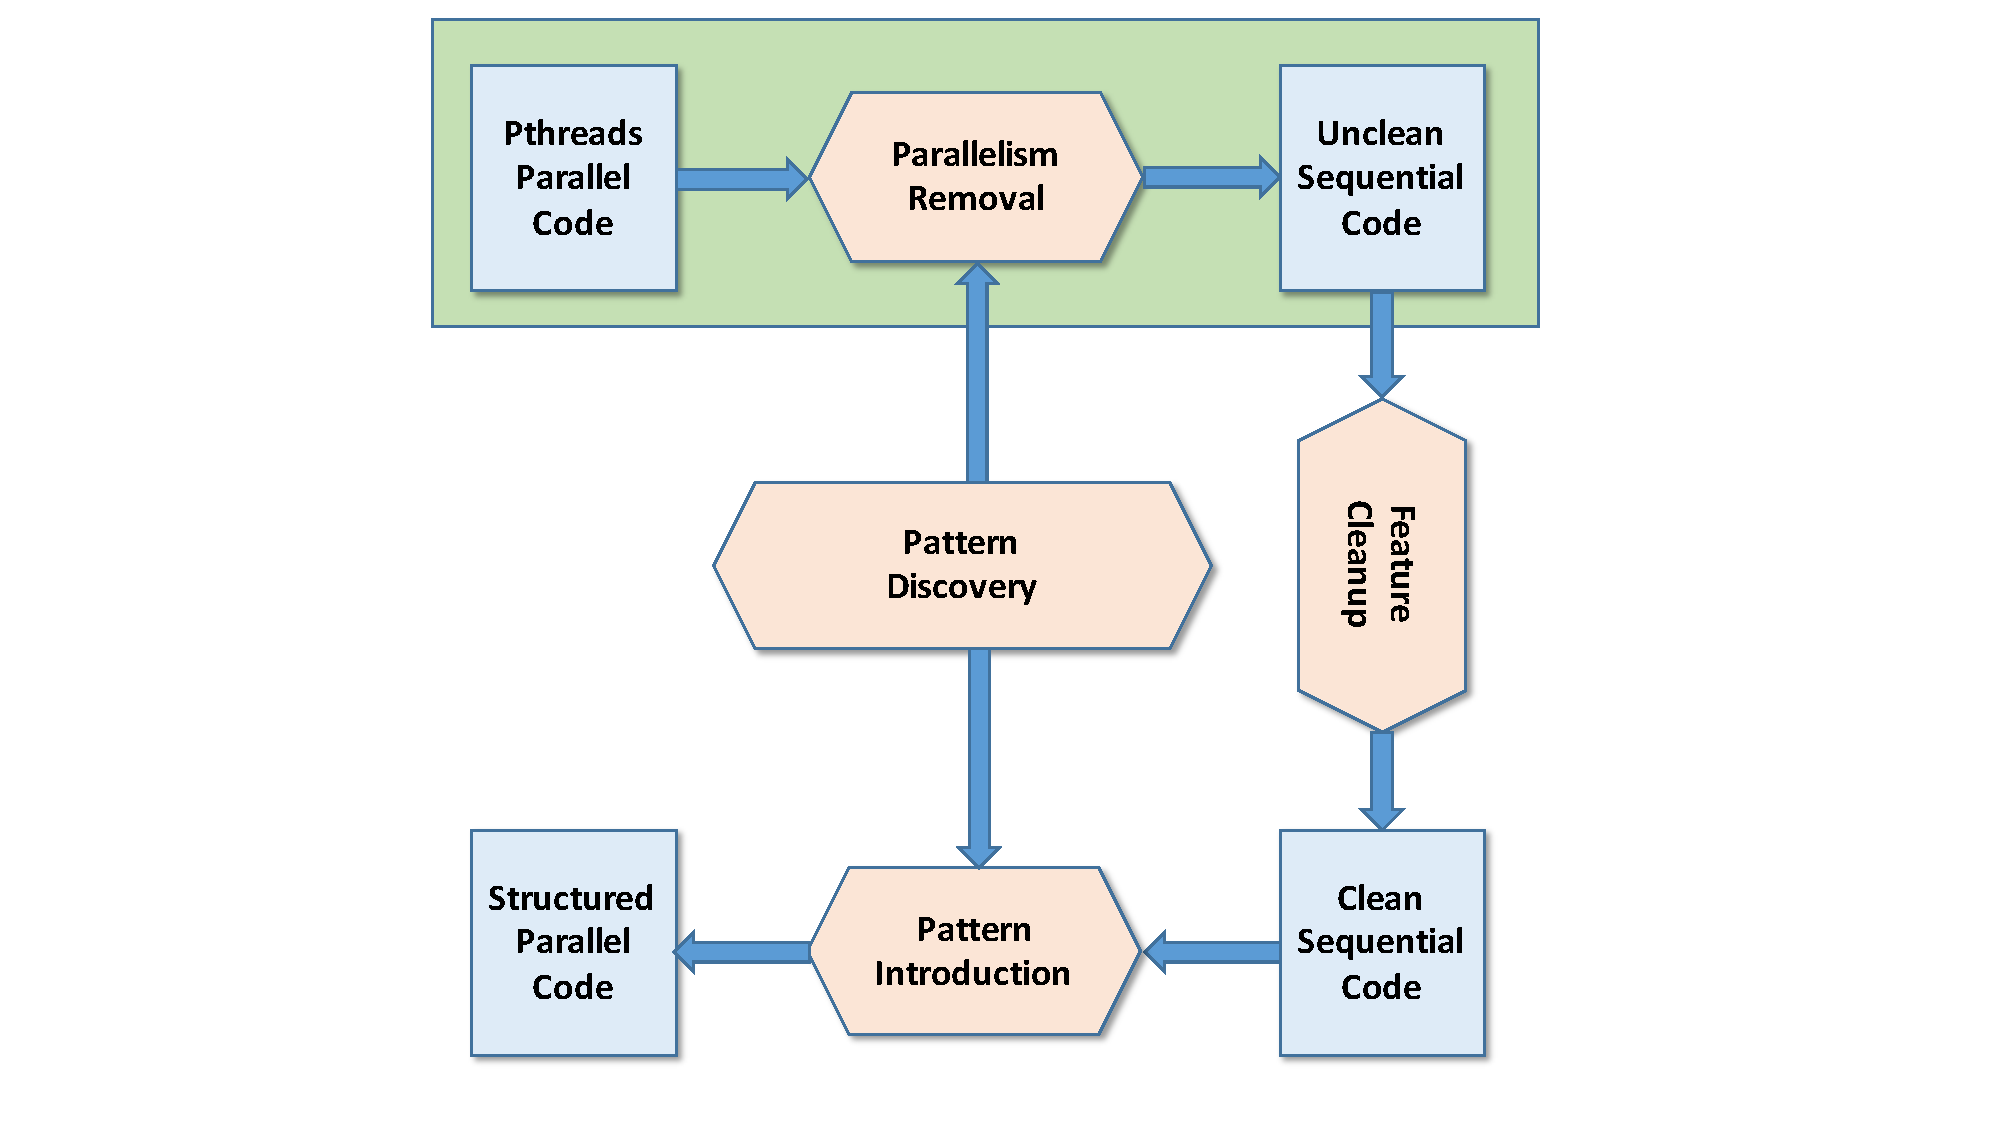
\includegraphics[width=0.5\textwidth]{SoftRest.pdf}
  \end{center}
  \vspace{-0.5cm}
  \caption{Software Restoration Process}
  \label{fig:SoftRest}
  \end{figure}

Legacy-parallel code, written in ad-hoc way using low level parallel libraries such as \emph{pthreads}, is still very much present in various software repositories and projects. This code was usually developed before the libraries and programming models that allow structured parallelisation (such as the ones mentioned in Section~\ref{XX}) were developed, and was usually written by parallelism experts and tailored to very specific hardware. This makes it very hard to maintain that code, an increasing important feature in software engineering, or to port it to new architectures. 

It would be ideal if every legacy-parallel application could be refactored into structured parallel programs, written using high-level parallel pattern libraries, ensuring good performance, maintainability and portability. However, for this to be possible, it is necessary that a well-defined underlying pattern of parallelism actually exists in the code, which can be exploited by instances of patterns. This is not always the case. However, in substantial number of cases, the parallelism in the application is an instance of one of the common patterns, such as farm, pipeline, workpool or stencil. In these cases, it should be possible, automatically or semi-automatically, to \emph{replace} unstructured parallelism with its structured (patterned) equivalent.   

\emph{Software restoration} is a methodology to transform a legacy-parallel code into a parallel patterned code, possibly with the addition of concurrency. It is based on software refactoring technology for semi-automatic, under the programmer's guidance, code-to-code transformation and supported by static and dynamic code analysis in the form of \emph{pattern discovery} to identify parts of the code that could be trasnformed into instances of parallel patterns. In the software restoration, code goes through different phases and it is usually necessary to remove ad-hoc parallelism and associated data structures in order to get the code into a \emph{clean state}, where instances of parallel patterns can be introduced. 

The overall software restoration process is depicted in Figure~\ref{fig:SoftRest}. We will use the Matrix Mulitplication benchmark as a running example to demonstrate the whole process. It involves the following steps.

\paragraph{Parallelism Removal.}
We start with a legacy-parallel application, written using one of the low level threading libraries. For the purposes of this paper, we will assume that the code is written using the \emph{pthreads} library, but the principle is the same with the similar libraries such as \emph{cilk} or \emph{MPI}. The initial step in software restoration is to do \emph{initial pattern discovery} first step in restoration is running an initial pattern discovery to discover i) parts of the threaded code that correspond to instances of parallel patterns; and, ii) parts of the threaded code that represent concurrent computations. It is necessary to know which threaded code is concurrent, as turning these portions of code into sequential code can lead to deadlocks in the code, and therefore prevent correct restoration. Pattern discovery is required to, firstly, mark the parts of the code that are of interest to restoration and, secondly, to drive the kind of transformations that are applied in the further steps.

In the Matrix Multiplication example, the following part of the code is source of parallelism, and the parallelism is of \emph{parallel farm} type. There is no additional concurrency, so we can remove all threaded code without restriction.

\begin{lstlisting}[linewidth=\columnwidth,language=C++,basicstyle=\tiny]
double **a;
double **b;
double **res;

int dim;
int thread_count;

typedef struct {
  int row_start;
  int row_end;
} input_data;

static void * func (void* arg)
{
  input_data *input = (input_data *)arg;
  unsigned int i;
  for (i = input->row_start; i < input->row_end; i++) {
          multiply_row_by_matrix(a, i, b, res);
  }

  return (void *)0;
}

void threads_create()
{
  pthread_attr_t attr;
  int status;

  threads = (pthread_t *) malloc (sizeof(pthread_t) * nr);

  status = pthread_attr_init(&attr);
  if (status != 0)
    std::cout << "Init attributes object" << std::endl;

  ...
  for (unsigned int ti = 0; ti < nr; ti++) {
    /* Setting some generic parameters for each thread */
    in[thread_ind].row_start = count;
    in[thread_ind].row_end = count + chunk;
    count += chunk;

    status = pthread_create(&threads[ti], 
                            &attr, &func, &in[ti]);
    if (status != 0)
      handle_error("Creating thread failed!");

  }
}
    \end{lstlisting}
    
    
  %  \item \emph{Parallelism removal.} 
  
  The first code transformation phase is \emph{parallelism removal}. Here, we remove parts of the threaded code  that are safe to remove (that is, all except the parts identified as concurrent computations during pattern discovery), and replace them with their sequential equivalents. For example, if a \emph{farm} pattern is applied to an operation over an input array (as is the case with Matrix Multiplication), we replace it with a  sequential loop that iterates the operation over the input array. In this way we get the sequential application with the same semantics as the original parallel one. In the case of Matrix Multiplication, we get the following code:
    
\begin{lstlisting}[linewidth=\columnwidth,language=C++,basicstyle=\tiny]
void threads_create()
{
  pthread_attr_t attr;
  int status;   

  threads = (pthread_t *) malloc (sizeof(pthread_t) * nr);

  status = pthread_attr_init(&attr);
  if (status != 0)
    std::cout << "Init attributes object" << std::endl;

  ...
  for (unsigned int ti = 0; ti < nr; ti++) {
    /* Setting some generic parameters for each thread */
    in[thread_ind].row_start = count;
    in[thread_ind].row_end = count + chunk;
    count += chunk;

    func(&in[ti]);
  }
}
\end{lstlisting}

\paragraph{Feature Cleanup.}
   The previous step removes all the parallelism creation and managing constructs from the legacy-parallel code. However, some artifacts of the initial parallelisation may still remain in the code. These can be, for example, queues between stages of the pipeline computation. In addition, the original data structures over which parallelism is applied (e.g.~an array or a tree in the \emph{farm} pattern) might have been restructured in some way to accomodate for a particular type of parallelism applied. All these artifacts can get in way of introducing structured parallelism in the code and can, furthermore, prevent exploring alternative alternative parallelisations (e.g.~using different combinations of patterns) of the code. Therefore, the next step in restoration is to get rid of the remaining artifacts of the initial ad-hoc parallelisation, to get the code as close as is possible to its initial, sequential state. This means removing intermediate buffers, queues and locks, and also possibly flattening data structures to which parallelism has been applied. 
  
   In the Matrix Multiplication example that we are considering, we can see that in the version with removed parallelism, the loop does not iterate over the elements of the input arrays (matrices \lstinline{a} or \lstinline{b}), but over the chunks of indices, lower and upper bound of each is stored into the \lstinline{in} data structure. This is necessary for manual parallelisation using the \lstinline{pthread} library, as there we need to explicitly divide work into chunks for each thread. However, in structured parallelisations using \lstinline{Intel TBB} or \lstinline{OpenMP} libraries, the underlying scheduler can take care of dividing work between threads, and this can be done even dynamically while the application is executing to determine most optimal work allocation. Therefore, it is better to get rid of the manual work chunking and restore the version where the main worker function iterates over the whole matrix \lstinline{a}:
   
   \begin{lstlisting}[linewidth=\columnwidth,language=C++,basicstyle=\tiny]
void threads_create()
{
  ...
  for (unsigned int i=0; i<dim; i+) {
    multiply_row_by_matrix(a, i, b, res);
  }
}
   \end{lstlisting}
   
   \paragraph{Parallelism Introduction.}
    Finally, once the code is restored into the state that is as close to the starting sequential version as possible, further pattern discovery analysis can be made on it, as the feature cleanup transformations, and especially flattening of data structures and elimination of intermediate buffers/queues, might result in the code that has additional instances of parallel patterns that were not detected on the original, legacy-parallel code. After that, we introduce instances of parallel patterns into now-clean sequential code. This is again done using the refactoring technology, where parts of the sequential code are replaced by calls to the functions from the high-level pattern libraries such as \lstinline{Intel TBB} or \lstinline{OpenMP}. 
    
    In the case of Matrix Multiplication, and using refactorings to introduce \lstinline{Intel TBB} patterns, we obtain the following code:
 
 \begin{lstlisting}[linewidth=\columnwidth,language=C++,basicstyle=\tiny]
 class MultiplyRowsMatrixTBB {
  double **mat1;
  double **mat2;
  double **res;
public:
  void operator() (const blocked_range<size_t>& r) const {
    for (size_t i=r.begin(); i!=r.end(); i++) {
      multiply_row_by_matrix(a, i, b, res);
    }
  }
  MultiplyRowsMatrixTBB(double **mat1, double **mat2, double **res)
    : mat1(mat1), mat2(mat2), res(res)
  {}
};

void threads_create()
{
  int status;
  parallel_for(blocked_range<size_t>(0,dim), 
               MultiplyRowsMatrixTBB(a, b, res));
}
\end{lstlisting}
    
    
    %\item \emph{Parallelism removal}. We start with a legacy-parallel application, written using \lstinline{pthreads} library. The first step in restoration is running an initial analysis to 
%\end{itemize}



\section{Refactorings to Eliminate Parallelism}
\subsection{Threads Removal}
\subsection{Pipeline Parallelism Removal}

\section{Use Cases}

\begin{figure}
\begin{tabular}{|c|c|c|c|c|c|}
\hline
\textbf{Use Case} & \textbf{Existing Par.} & \textbf{Discovered Par.} & \textbf{Removal Works?} & \textbf{Feature Cleanup Needed?} & \textbf{Benefit} \\ \hline \hline
Matrix Multiplication & Farm & Farm & Yes & Sort of & Speedup \\
PgPry & Pipeline + Farm & & No & Yes & \\
Bvi Plus & Concurrency & & No & &  \\
TvPvr Daemon & Concurrency & & No & &  \\
Fluid Animation & Farm & & Yes & Yes & \\ \hline
Blackscholes & Farm & &  & No & \\
Bodytrack & Workpoolish & & No & Probably & \\
Swaptions & Farm & & & No & \\
Frequency Mining & Many Farms & & & & \\ \hline
Ferret & Pipeline & & & & \\
X264 & Pipeline & & & & \\
Dedup & Pipeline & & & & \\
\hline


\end{tabular}
\end{figure}


\subsection{Matrix Multiplication}
\subsection{PgPry}

\section{Related Work}

% Semi-automatic Extraction and Exploitation of Hierarchical Pipeline Parallelism Using Profiling Information
\cite{Tournavitis:2010:SEE:1854273.1854321}

% Towards a Compiler Analysis for Parallel Algorithmic Skeletons
\cite{vonKoch:2018:TCA:3178372.3179513}

\section{Conclusions and Future Work}

%\input{samplebody-conf}

\bibliographystyle{ACM-Reference-Format}
\bibliography{main}

\end{document}
